%=============================================================================
% High-Speed Ethernet: From the OSI Model to 400G
%
% A single-file, self-contained learning guide covering networking
% fundamentals, Ethernet (MAC/PHY), and the 400G Ethernet architecture.
%
% Build with:  pdflatex ethernet_public.tex   (run twice for TOC/refs)
%
% Requires the standard "tufte-book" class (bundled with TeX Live / MiKTeX).
% No external fonts, images, or bibliography files are needed.
%=============================================================================

\documentclass[openany]{tufte-book}

%---------------------------------------
% Document metadata
%---------------------------------------
\newcommand\proptitle{High-Speed Ethernet: From the OSI Model to 1.6T}
\newcommand\propnumber{Learning Notes}
\newcommand\shorttitle{High-Speed Ethernet}

%---------------------------------------
% Packages
% (tufte-book already loads natbib, graphicx, hyperref, geometry, etc.)
%---------------------------------------
\usepackage{amsmath}
\usepackage{amssymb}
\usepackage{xcolor}
\usepackage{colortbl}
\usepackage{booktabs}
\usepackage{tabularx}
\usepackage{array}
\usepackage{ragged2e}
\usepackage{tikz}
\usetikzlibrary{positioning,arrows.meta,shapes,calc,shadows}
\usepackage{multicol}
\usepackage{subcaption}
\usepackage{enumitem}
\usepackage{url}
\usepackage{setspace}
\usepackage{framed}

% Map the few Unicode symbols used in the text so the file compiles with
% pdflatex (as well as xelatex/lualatex).
\usepackage{newunicodechar}
\newunicodechar{→}{\ensuremath{\rightarrow}}
\newunicodechar{×}{\ensuremath{\times}}
\newunicodechar{÷}{\ensuremath{\div}}
\newunicodechar{↔}{\ensuremath{\leftrightarrow}}

%---------------------------------------
% Fonts
%
% This public edition uses the tufte-book default fonts so it compiles
% anywhere with a standard TeX distribution (pdflatex, no local font files).
% \headingfont is defined as a sans-serif fallback so heading/header macros
% below keep working.
%---------------------------------------
\newcommand{\headingfont}{\sffamily}

%---------------------------------------
% Spacing and layout
%---------------------------------------
\setlength{\parskip}{0.2em}
\linespread{0.95}

\setlist[itemize]{
    leftmargin=*,
    itemsep=0.2em,
    parsep=0em,
    topsep=0.2em
}

%---------------------------------------
% Header / footer
%---------------------------------------
\usepackage{fancyhdr,lastpage}

\fancyhf{}
\fancyhead[L]{\headingfont\small{}}
\fancyhead[C]{\headingfont\small{\shorttitle}}
\fancyhead[R]{\headingfont\small{\propnumber}}
\cfoot{\headingfont{Page \thepage\ of \pageref{LastPage}}}
\renewcommand{\headrulewidth}{0pt}
\renewcommand{\footrulewidth}{0pt}

\fancypagestyle{firststyle}{
    \fancyhf{}
    \fancyhead[C]{\headingfont\small{\shorttitle}}
    \fancyhead[R]{\headingfont\small{\propnumber}}
    \cfoot{\headingfont{Page \thepage\ of \pageref{LastPage}}}
    \renewcommand{\footrulewidth}{0pt}
}

%---------------------------------------
% Title
%---------------------------------------
\title{\proptitle}
\author{}
\date{}

%---------------------------------------
% Table of contents depth
%---------------------------------------
\setcounter{tocdepth}{2}

%---------------------------------------
% Re-enable \subsubsection
%
% tufte-book intentionally disables \subsubsection. This guide uses it, so we
% redefine it as an unnumbered bold heading that still lists in the TOC.
%---------------------------------------
\makeatletter
\renewcommand{\subsubsection}[1]{%
  \par\medskip\noindent\textbf{#1}\par\nopagebreak\smallskip
  \addcontentsline{toc}{subsubsection}{#1}%
}
\makeatother

\begin{document}

\maketitle
\tableofcontents

% ============================================================================
% CHAPTER 0A: OSI MODEL AND NETWORKING BASICS
% ============================================================================

\chapter{Network Fundamentals: The OSI Model}

\section{Introduction}

This chapter introduces the foundational networking concepts you need to understand high-speed Ethernet. We'll cover the OSI model and how different network layers work together.

Think of this as learning the alphabet before reading. Once you understand these basics, the more complex 400G and 800G architectures will make much more sense.

\section{The OSI Model: Understanding Network Layers}

Computer networks are organized into layers, each with specific responsibilities. The \textbf{OSI (Open Systems Interconnection) Model} divides networking into seven layers.

\subsection{The Seven Layers}

Think of the OSI model as a stack of responsibilities, where each layer provides services to the layer above it:

\begin{fullwidth}
\begin{table}
\centering
\begin{tabular}{clp{8cm}}
\toprule
\textbf{Layer} & \textbf{Name} & \textbf{Function} \\
\midrule
7 & Application & User applications (web browsers, email) \\
6 & Presentation & Data formatting, encryption \\
5 & Session & Connection management \\
4 & Transport & End-to-end delivery (TCP, UDP) \\
3 & Network & Routing between networks (IP addresses) \\
\rowcolor{yellow!30}
2 & Data Link & Frame delivery on local network (MAC addresses) \\
\rowcolor{yellow!30}
1 & Physical & Electrical/optical signals on wire/fiber \\
\bottomrule
\end{tabular}
\caption{The OSI Seven-Layer Model. Ethernet operates at Layers 1 and 2 (highlighted).}
\end{table}
\end{fullwidth}

\textbf{Ethernet operates at Layers 1 and 2}---the Physical and Data Link layers. This is crucial: Ethernet doesn't care about IP addresses (Layer 3) or TCP connections (Layer 4). It simply moves frames of data between devices on the same local network.

\subsection{Data Flow Example}

Let's trace how data moves through the layers when you load a webpage:

\begin{enumerate}
\item \textbf{Application Layer (7)}: Your web browser requests a webpage
\item \textbf{Transport Layer (4)}: TCP breaks the request into segments
\item \textbf{Network Layer (3)}: IP adds routing information (IP addresses)
\item \textbf{Data Link Layer (2)}: \textbf{Ethernet adds MAC addresses and creates frames}
\item \textbf{Physical Layer (1)}: \textbf{Ethernet converts frames to electrical/optical signals}
\end{enumerate}

The receiving computer reverses this process, moving up through the layers until your webpage appears in the browser.

\section{Why Layers Matter for High-Speed Ethernet}

Understanding the OSI model helps you see where high-speed Ethernet fits in the networking stack:

\begin{itemize}
\item \textbf{Layer 2 (Data Link)}: MAC sublayer creates Ethernet frames
\item \textbf{Layer 1 (Physical)}: PHY sublayers (PCS, PMA, PMD) convert frames to optical signals
\end{itemize}

The beauty of this layered approach is that higher layers (IP, TCP, applications) don't need to know whether they're running over 1G, 10G, 400G, or 800G Ethernet. The interface between layers remains consistent.

% ============================================================================
% CHAPTER 0B: ETHERNET FUNDAMENTALS
% ============================================================================

\chapter{Ethernet Fundamentals: MAC and PHY}

\section{Introduction}

Now that you understand the OSI model, let's dive into Ethernet itself. This chapter covers the MAC layer, Ethernet frames, and the PHY architecture that makes high-speed data transmission possible.

\section{Layer 2: The MAC Sublayer}

\textbf{MAC (Media Access Control)} is the lower portion of Layer 2. It handles addressing (every interface has a unique 48-bit MAC address like \texttt{00:1A:2B:3C:4D:5E}), framing (wraps data in Ethernet frames with headers and error detection), and media access control (manages when devices can transmit). The MAC is implemented in the host processor (CPU) or network ASIC and is software-accessible---drivers and operating systems interact with it to send/receive frames.

\subsection{Ethernet Frame Structure}

When the MAC layer receives data from Layer 3, it creates an Ethernet frame:

\begin{fullwidth}
\begin{figure}
\centering
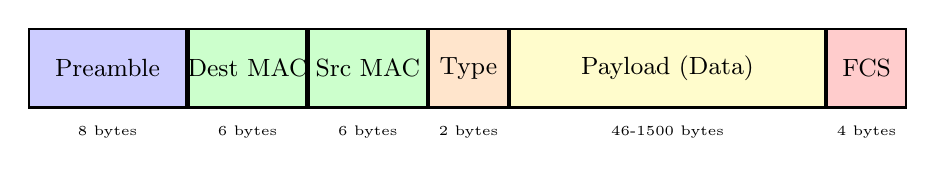
\begin{tikzpicture}[
    box/.style={rectangle, draw=black, thick, minimum height=1cm, anchor=west},
    label/.style={font=\small}
]

\node[box, fill=blue!20, minimum width=2cm] (preamble) at (0,0) {};
\node[label] at (preamble.center) {Preamble};
\node[below=0.1cm of preamble.south, font=\tiny] {8 bytes};

\node[box, fill=green!20, minimum width=1.5cm, right=0cm of preamble.east, anchor=west] (dest) {};
\node[label] at (dest.center) {Dest MAC};
\node[below=0.1cm of dest.south, font=\tiny] {6 bytes};

\node[box, fill=green!20, minimum width=1.5cm, right=0cm of dest.east, anchor=west] (src) {};
\node[label] at (src.center) {Src MAC};
\node[below=0.1cm of src.south, font=\tiny] {6 bytes};

\node[box, fill=orange!20, minimum width=1cm, right=0cm of src.east, anchor=west] (type) {};
\node[label] at (type.center) {Type};
\node[below=0.1cm of type.south, font=\tiny] {2 bytes};

\node[box, fill=yellow!20, minimum width=4cm, right=0cm of type.east, anchor=west] (payload) {};
\node[label] at (payload.center) {Payload (Data)};
\node[below=0.1cm of payload.south, font=\tiny] {46-1500 bytes};

\node[box, fill=red!20, minimum width=1cm, right=0cm of payload.east, anchor=west] (fcs) {};
\node[label] at (fcs.center) {FCS};
\node[below=0.1cm of fcs.south, font=\tiny] {4 bytes};

\end{tikzpicture}
\caption{Ethernet Frame Structure. The MAC layer creates this frame format.}
\end{figure}
\end{fullwidth}

\textbf{Frame Components:}
\begin{itemize}
\item \textbf{Preamble}: Synchronization pattern (7 bytes of 0x55 + 1 byte SFD)
\item \textbf{Destination MAC}: Hardware address of recipient
\item \textbf{Source MAC}: Hardware address of sender  
\item \textbf{EtherType}: Protocol identifier (0x0800 = IPv4, 0x86DD = IPv6)
\item \textbf{Payload}: Actual data (46-1500 bytes)
\item \textbf{FCS}: Frame Check Sequence (CRC32 checksum for error detection)
\end{itemize}

\section{The Ethernet PHY: Physical Layer Overview}

The \textbf{PHY (Physical Layer)} converts MAC frames into electrical or optical signals for transmission. The PHY is subdivided into multiple sublayers:

\begin{itemize}
\item \textbf{RS (Reconciliation Sublayer)}: Adapts MAC to PHY
\item \textbf{PCS (Physical Coding Sublayer)}: Encoding, FEC, scrambling
\item \textbf{PMA (Physical Medium Attachment)}: Serialization, lane alignment
\item \textbf{PMD (Physical Medium Dependent)}: Electrical/optical signaling
\end{itemize}

Between MAC and PCS, GMII-style interfaces (e.g., 400GMII, 800GMII) use wide parallel buses inside the chip for easier logic and lower power.

\subsection{Physical Implementation: Chip Boundaries}

Understanding \textbf{where these functions physically exist} is important. The example below shows a representative 400G optical-module implementation.

\begin{fullwidth}
\begin{figure}
\centering
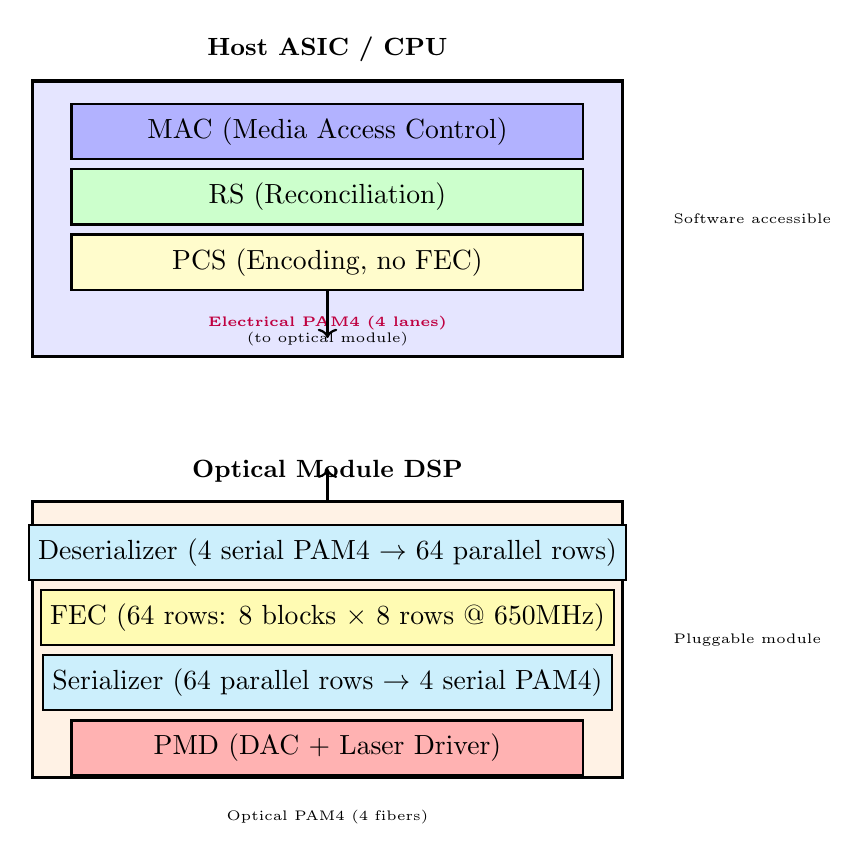
\begin{tikzpicture}[
    chip/.style={rectangle, draw=black, very thick, minimum height=3.5cm, anchor=north},
    layer/.style={rectangle, draw=black, thick, minimum width=6.5cm, minimum height=0.7cm, anchor=north},
    arrow/.style={->, thick}
]

% Host ASIC
\node[chip, fill=blue!10, minimum width=7.5cm] (asic) at (0,0) {};
\node[above=0.1cm of asic.north, font=\small\bfseries] {Host ASIC / CPU};

\node[layer, fill=blue!30, below=0.3cm of asic.north] (mac) {MAC (Media Access Control)};
\node[layer, fill=green!20, below=0.1cm of mac.south] (rs) {RS (Reconciliation)};
\node[layer, fill=yellow!20, below=0.1cm of rs.south] (pcs) {PCS (Encoding, no FEC)};

\node[below=0.2cm of pcs.south, font=\tiny\bfseries, color=purple] {Electrical PAM4 (4 lanes)};
\node[below=0.4cm of pcs.south, font=\tiny] {(to optical module)};

% Optical Module
\node[chip, fill=orange!10, minimum width=7.5cm, below=1.8cm of asic.south] (module) {};
\node[above=0.1cm of module.north, font=\small\bfseries] {Optical Module DSP};

\node[layer, fill=cyan!20, below=0.3cm of module.north] (des) {Deserializer (4 serial PAM4 $\rightarrow$ 64 parallel rows)};
\node[layer, fill=yellow!30, below=0.1cm of des.south] (fec) {FEC (64 rows: 8 blocks $\times$ 8 rows @ 650MHz)};
\node[layer, fill=cyan!20, below=0.1cm of fec.south] (ser) {Serializer (64 parallel rows $\rightarrow$ 4 serial PAM4)};
\node[layer, fill=red!30, below=0.1cm of ser.south] (pmd) {PMD (DAC + Laser Driver)};

\node[below=0.3cm of pmd.south, font=\tiny] {Optical PAM4 (4 fibers)};

\draw[arrow] (pcs.south) -- ++(0,-0.6cm);
\draw[arrow] (module.north) -- ++(0,0.4cm);

% Labels positioned to the right
\node[right=0.5cm of asic.east, anchor=west, font=\tiny] {Software accessible};
\node[right=0.5cm of module.east, anchor=west, font=\tiny] {Pluggable module};

\end{tikzpicture}
\caption{A representative 400G architecture. Deserializer: 4 serial PAM4 $\rightarrow$ 64 parallel rows. FEC: 64 rows (8 blocks $\times$ 8 rows $\times$ 10 bits). Each block = 80 bits processed every 1.5ns.}
\end{figure}
\end{fullwidth}

\marginnote{Each 400G DSP has 8 parallel FEC blocks. Each block = 80 bits (8 RS-FEC symbols $\times$ 10 bits). FEC block rate: 53.125 Gb/s. Total per DSP: 8 $\times$ 53.125 Gb/s = 425 Gb/s (400 Gb/s payload + FEC).}

\textbf{Key Points:}
\begin{itemize}
\item \textbf{Host ASIC}: MAC, RS, PCS (encoding, scrambling, no FEC)
\item \textbf{Module receives}: 4 serial PAM4 lanes $\times$ 106.25 Gb/s = 425 Gb/s
\item \textbf{Deserializer}: Converts 4 serial lanes $\rightarrow$ 64 parallel rows (8 blocks $\times$ 8 rows)
\item \textbf{FEC}: Processes 64 rows in parallel, organized as 8 blocks of 80 bits each
\item \textbf{Serializer}: Converts 64 parallel rows $\rightarrow$ 4 serial lanes
\item \textbf{PMD}: Converts electrical PAM4 $\rightarrow$ optical PAM4 via DAC and laser driver
\end{itemize}

\section{Summary}

This chapter covered the essential Ethernet concepts:
\begin{itemize}
\item MAC layer creates frames with addressing and error detection
\item PHY sublayers transform frames into optical signals
\item The architecture splits between host ASIC (MAC/PCS) and optical module (FEC/PMD)
\end{itemize}

In the next chapter, we'll dive deeper into the 400G architecture and see how data flows through each sublayer.

% ============================================================================
% CHAPTER 1: 400G ETHERNET ARCHITECTURE
% ============================================================================

\chapter{400G Ethernet: The Foundation}

\section{Introduction}

This chapter focuses on 400G Ethernet because it's the foundation for 800G---which is literally two 400G systems running in parallel. 400G operates at 400 Gb/s payload rate (425 Gb/s with FEC overhead), uses 4 physical lanes at 106.25 Gb/s each with PAM4 modulation, and employs RS(544,514) FEC for error correction. Data flows: MAC → 400GMII (64-bit parallel bus) → PCS (encoding, FEC) → PMA (serialization) → 400GAUI-4 (4 electrical lanes) → PMD (optical signaling).

\section{The 400GMII Interface}

\textbf{400GMII (400 Gigabit Media Independent Interface)} is a 64-bit parallel bus inside the chip between the MAC and PCS. It transfers 64 bits per clock cycle at ~6.25 GHz, giving 400 Gb/s throughput. Parallel buses work well inside chips (short distances, lower power) but not between chips (skew problems), which is why external interfaces use serial lanes.

\section{PCS: Encoding and Preparation}

\subsection{The PCS Flow (in Host ASIC)}

The PCS in the host ASIC prepares data for transmission but does NOT include FEC (FEC is in the module).

\textbf{PCS operations (streaming, real-time)}:

64-bit chunks from MAC → encoded to 66-bit blocks (adds 2-bit sync headers) → four 66-bit blocks combined into 257-bit blocks (compresses sync headers) → scrambled → serialized to 4 PAM4 lanes at 106.25 Gb/s each.

\textbf{Output from host ASIC}: 4 serial PAM4 lanes × 106.25 Gb/s = 425 Gb/s (includes overhead for FEC that will be added in the module).

\subsection{64B/66B Encoding: Adding Sync Headers}

Before transcoding can happen, the MAC's 64-bit words must be encoded into
66-bit blocks. This is the first transformation.

\textbf{The MAC delivers two things per clock cycle}:
\begin{itemize}
\item \textbf{TXD[63:0]}: 64 bits of data (8 octets in parallel)
\item \textbf{TXC[7:0]}: 8 control bits, one per octet (1 = this octet is a
control character, 0 = data)
\end{itemize}

The 64B/66B encoder examines these 72 bits and produces a 66-bit block with a
\textbf{2-bit sync header} prepended:

\begin{itemize}
\item \textbf{Sync header \texttt{01}}: This block carries \textit{data only}.
All 8 octets are payload data. The 64 payload bits follow directly.
\item \textbf{Sync header \texttt{10}}: This block carries \textit{control
information} (or a mix of control and data). The 64 payload bits encode the
specific control pattern (idle, start-of-frame, end-of-frame, etc.).
\end{itemize}

\marginnote{The sync header is never \texttt{00} or \texttt{11}. Those patterns
are illegal and would indicate a framing error. The receiver uses this
constraint to lock onto block boundaries in the serial stream.}

\textbf{Why only 2 bits?} The receiver needs to find block boundaries in a
continuous serial bit stream. With a 2-bit header that is always \texttt{01}
or \texttt{10}, the receiver can scan for these patterns and lock on. The
overhead is only $2/66 = 3.03\%$, which is very efficient.

\textbf{Overhead calculation}:
\begin{equation}
\text{Efficiency} = \frac{64}{66} = 96.97\%
\end{equation}
\begin{equation}
\text{Line rate needed} = \frac{400 \text{ Gb/s}}{0.9697} \approx 412.5 \text{ Gb/s}
\end{equation}

So after 64B/66B encoding, the raw bit rate rises from 400 Gb/s to about
412.5 Gb/s. The remaining overhead (to reach 425 Gb/s) comes from FEC.

\subsection{Transcoding: From 66-bit Blocks to 257-bit Blocks}

\textbf{Transcoding is the process of combining four consecutive 66-bit blocks
into a single 257-bit block.} This is also called 256B/257B encoding in the
IEEE 802.3 standard.

\subsubsection{Why Transcode at All?}

There are three reasons, each important:

\textbf{Reason 1: Reduce sync header overhead.}

Four 66-bit blocks contain $4 \times 2 = 8$ sync header bits. After
transcoding, the 257-bit block has only 1 sync bit. We went from 8 bits of
overhead to 1 bit of overhead for the same amount of payload:

\begin{equation}
\text{Before: } \frac{8 \text{ sync bits}}{264 \text{ total bits}} = 3.03\%
\text{ overhead}
\end{equation}
\begin{equation}
\text{After: } \frac{1 \text{ sync bit}}{257 \text{ total bits}} = 0.39\%
\text{ overhead}
\end{equation}

\textbf{Reason 2: Create a payload size that aligns with FEC symbols.}

The RS-FEC code works with \textbf{10-bit symbols}. The 256-bit payload of a
257-bit block has a clean mathematical relationship with 10:

\begin{equation}
\text{LCM}(256, 10) = 1280 \text{ bits}
\end{equation}

Every 5 blocks ($5 \times 256 = 1280$ bits), the payload divides into exactly
128 RS-FEC symbols with no remainder. This means no partial symbols, no
wasted bits, and simpler hardware.

\textbf{Reason 3: Larger blocks are more efficient for FEC processing.}

FEC encoders work on fixed-size codewords. Larger input blocks mean fewer
block boundaries to manage, less framing overhead, and better utilization of
the FEC encoder's pipeline.

\subsubsection{Exactly What Happens to Every Bit}

Let's trace every bit through the transcoding process with a concrete example.

\textbf{Input: Four consecutive 66-bit blocks}

\begin{fullwidth}
\begin{table}
\centering
\small
\begin{tabular}{llll}
\toprule
\textbf{Block} & \textbf{Sync Header (bits 65:64)} & \textbf{Payload (bits 63:0)} & \textbf{Total} \\
\midrule
Block A & \texttt{01} (data block) & \texttt{D$_A$[63:0]} & 66 bits \\
Block B & \texttt{01} (data block) & \texttt{D$_B$[63:0]} & 66 bits \\
Block C & \texttt{10} (control block) & \texttt{D$_C$[63:0]} & 66 bits \\
Block D & \texttt{01} (data block) & \texttt{D$_D$[63:0]} & 66 bits \\
\midrule
\textbf{Total input} & 8 sync bits & 256 payload bits & \textbf{264 bits} \\
\bottomrule
\end{tabular}
\caption{Four 66-bit blocks entering the transcoder. Each has a 2-bit sync
header and 64 bits of payload.}
\end{table}
\end{fullwidth}

\textbf{Step 1: Strip the four 2-bit sync headers.}

The transcoder extracts the four sync headers:
\begin{itemize}
\item Header$_A$ = \texttt{01}
\item Header$_B$ = \texttt{01}
\item Header$_C$ = \texttt{10}
\item Header$_D$ = \texttt{01}
\end{itemize}

These 8 bits are \textit{removed} from the payload stream. The four 64-bit
payloads remain: $D_A$, $D_B$, $D_C$, $D_D$.

\textbf{Step 2: Concatenate the four 64-bit payloads.}

The payloads are joined end-to-end in order:

\begin{equation}
\text{256-bit payload} = D_A[63:0] \,\|\, D_B[63:0] \,\|\, D_C[63:0] \,\|\, D_D[63:0]
\end{equation}

where $\|$ means concatenation. The result is a flat 256-bit word. No bits are
reordered, no bits are dropped---just four 64-bit words placed back-to-back.

\textbf{Step 3: Encode the four sync headers into one new sync bit.}

This is the key step. The four 2-bit headers are \textit{compressed} into a
single 1-bit sync header using a lookup table defined in IEEE 802.3 Clause 82.

The valid sync header patterns and their encodings are:

\begin{fullwidth}
\begin{table}
\centering
\begin{tabular}{lllll}
\toprule
\textbf{Header$_A$} & \textbf{Header$_B$} & \textbf{Header$_C$} &
\textbf{Header$_D$} & \textbf{New 1-bit sync} \\
\midrule
\texttt{01} & \texttt{01} & \texttt{01} & \texttt{01} & \texttt{0} \\
\texttt{10} & \texttt{01} & \texttt{01} & \texttt{01} & \texttt{1} \\
\texttt{01} & \texttt{10} & \texttt{01} & \texttt{01} & \texttt{1} \\
\texttt{01} & \texttt{01} & \texttt{10} & \texttt{01} & \texttt{1} \\
\texttt{01} & \texttt{01} & \texttt{01} & \texttt{10} & \texttt{1} \\
\texttt{10} & \texttt{10} & \texttt{01} & \texttt{01} & \texttt{1} \\
\texttt{10} & \texttt{01} & \texttt{10} & \texttt{01} & \texttt{1} \\
\texttt{10} & \texttt{01} & \texttt{01} & \texttt{10} & \texttt{1} \\
\texttt{01} & \texttt{10} & \texttt{10} & \texttt{01} & \texttt{1} \\
\texttt{01} & \texttt{10} & \texttt{01} & \texttt{10} & \texttt{1} \\
\texttt{01} & \texttt{01} & \texttt{10} & \texttt{10} & \texttt{1} \\
\texttt{10} & \texttt{10} & \texttt{10} & \texttt{01} & \texttt{1} \\
\texttt{10} & \texttt{10} & \texttt{01} & \texttt{10} & \texttt{1} \\
\texttt{10} & \texttt{01} & \texttt{10} & \texttt{10} & \texttt{1} \\
\texttt{01} & \texttt{10} & \texttt{10} & \texttt{10} & \texttt{1} \\
\texttt{10} & \texttt{10} & \texttt{10} & \texttt{10} & \texttt{1} \\
\bottomrule
\end{tabular}
\caption{Sync header compression table. All-data (\texttt{01 01 01 01}) maps
to sync bit \texttt{0}. Any other valid combination maps to \texttt{1}. The
receiver uses this table in reverse to reconstruct the original four headers.}
\end{table}
\end{fullwidth}

\marginnote{The rule is simple: sync bit = \texttt{0} if all four input headers
are \texttt{01} (pure data), sync bit = \texttt{1} for any other valid
combination. The receiver reconstructs the original headers by reading the
payload's first few bits, which encode the specific pattern.}

In our example: headers are \texttt{01}, \texttt{01}, \texttt{10}, \texttt{01}
--- not all-data, so the new sync bit = \texttt{1}.

\textbf{But wait --- how does the receiver know \textit{which} of the 15
non-zero patterns was used?}

The answer is that the specific pattern is encoded into the \textbf{first 8
bits of the 256-bit payload} using a secondary encoding defined in the
standard. The receiver reads the sync bit first, then reads those first 8 bits
to determine the exact original header combination, then reconstructs all four
original 66-bit blocks.

\textbf{Step 4: Assemble the 257-bit block.}

The final 257-bit block is assembled as:

\begin{equation}
\underbrace{\text{sync}[0]}_{\text{1 bit}} \;\|\;
\underbrace{D_A[63:0] \,\|\, D_B[63:0] \,\|\, D_C[63:0] \,\|\, D_D[63:0]}_{\text{256 bits}}
= \textbf{257 bits}
\end{equation}

\textbf{Bit accounting summary}:

\begin{fullwidth}
\begin{table}
\centering
\begin{tabular}{lrrl}
\toprule
\textbf{Bits} & \textbf{Before} & \textbf{After} & \textbf{What happened} \\
\midrule
Sync headers & 8 bits (4 × 2) & 1 bit & Compressed via lookup table \\
Payload data & 256 bits (4 × 64) & 256 bits & Concatenated, unchanged \\
\midrule
\textbf{Total} & \textbf{264 bits} & \textbf{257 bits} & \textbf{7 bits saved} \\
\bottomrule
\end{tabular}
\caption{Bit accounting through transcoding. The 256 payload bits are
completely preserved. Only the 8 sync bits are compressed to 1.}
\end{table}
\end{fullwidth}

\subsubsection{Why 256 Bits of Payload is the Right Number}

The choice of 256 bits (not 128, not 512) is deliberate and connects directly
to the FEC design.

\textbf{The FEC symbol size is 10 bits.} The RS(544,514) code operates on
10-bit symbols. For the hardware to be simple, the payload size should have a
clean relationship with 10.

\textbf{256 and 10 share a useful LCM}:
\begin{equation}
\text{LCM}(256, 10) = 1280 \text{ bits} = 5 \text{ blocks} = 128 \text{ symbols}
\end{equation}

This means every 5 consecutive 257-bit blocks, the sync bits are stripped and
the 1280 payload bits divide into exactly 128 RS-FEC symbols with zero
remainder. The hardware never has to handle a partial symbol spanning a block
boundary.

\textbf{Compare to what 66-bit blocks would give}:
\begin{equation}
\text{LCM}(64, 10) = 320 \text{ bits} \quad \text{(manageable, but 64B/66B
overhead is higher)}
\end{equation}

The 256-bit payload is also a power of 2 ($256 = 2^8$), which simplifies
address generation and buffer sizing in hardware.

\subsubsection{The Complete Bit Flow: A Worked Example}

Let's trace 256 bits of actual data from MAC to 257-bit block, showing every
transformation.

\textbf{Starting point}: MAC delivers two 64-bit words (we'll trace 128 bits
for brevity, the pattern repeats):

\begin{itemize}
\item Word 1: \texttt{0xDEADBEEFCAFEBABE} (64 bits, all data, TXC = 0x00)
\item Word 2: \texttt{0x0102030405060708} (64 bits, all data, TXC = 0x00)
\end{itemize}

\textbf{After 64B/66B encoding}:
\begin{itemize}
\item Block 1: \texttt{01} + \texttt{0xDEADBEEFCAFEBABE} = 66 bits
\item Block 2: \texttt{01} + \texttt{0x0102030405060708} = 66 bits
\end{itemize}

Sync header is \texttt{01} for both because TXC = 0x00 (pure data).

\textbf{After collecting four blocks for transcoding}:

Assume blocks 3 and 4 are also pure data:
\begin{itemize}
\item Block 3: \texttt{01} + \texttt{0xAAAAAAAAAAAAAAAA} = 66 bits
\item Block 4: \texttt{01} + \texttt{0x5555555555555555} = 66 bits
\end{itemize}

\textbf{Transcoding step-by-step}:
\begin{enumerate}
\item Strip headers: \texttt{01}, \texttt{01}, \texttt{01}, \texttt{01}
\item All-data pattern → new sync bit = \texttt{0}
\item Concatenate payloads:
\begin{itemize}
\item Bits [255:192]: \texttt{0xDEADBEEFCAFEBABE}
\item Bits [191:128]: \texttt{0x0102030405060708}
\item Bits [127:64]:  \texttt{0xAAAAAAAAAAAAAAAA}
\item Bits [63:0]:    \texttt{0x5555555555555555}
\end{itemize}
\item Prepend sync bit \texttt{0}
\item \textbf{Result}: 257-bit block = \texttt{0} + 256 bits of payload
\end{enumerate}

\textbf{Key observation}: Every single payload bit from the MAC arrives
unchanged in the 257-bit block. The transcoder only manipulates the sync
headers --- the data itself is never modified.

\subsubsection{What the Receiver Does in Reverse}

On the receive side, the de-transcoder (also called the inverse transcoder)
reverses the process:

\begin{enumerate}
\item Read the 1-bit sync header of the 257-bit block
\item If sync = \texttt{0}: all four output blocks get header \texttt{01}
\item If sync = \texttt{1}: read the first 8 bits of the payload to determine
which of the 15 non-zero patterns applies, then assign the correct headers
\item Split the 256-bit payload back into four 64-bit chunks
\item Reconstruct four 66-bit blocks: header + 64-bit chunk for each
\item Pass the four 66-bit blocks to the 64B/66B decoder
\end{enumerate}

The 64B/66B decoder then strips the sync headers and reconstructs the original
TXD[63:0] and TXC[7:0] signals for the MAC.

\subsubsection{Overhead Comparison: Before and After Transcoding}

\begin{fullwidth}
\begin{table}
\centering
\begin{tabular}{lrrrr}
\toprule
\textbf{Format} & \textbf{Payload bits} & \textbf{Overhead bits} &
\textbf{Total bits} & \textbf{Overhead \%} \\
\midrule
Raw MAC data & 256 & 0 & 256 & 0\% \\
After 64B/66B (4 blocks) & 256 & 8 & 264 & 3.03\% \\
After transcoding (257b) & 256 & 1 & 257 & 0.39\% \\
\midrule
\textbf{Overhead reduction} & & \textbf{7 bits saved} & & \textbf{2.64\%
better} \\
\bottomrule
\end{tabular}
\caption{Overhead comparison. Transcoding reduces sync overhead from 3.03\% to
0.39\% for the same 256 bits of payload.}
\end{table}
\end{fullwidth}

\marginnote{The 0.39\% overhead from the 257-bit sync bit is so small that it
barely affects the line rate calculation. The dominant overhead in 400G comes
from FEC (5.8\%), not from encoding.}

\section{Module DSP: FEC and Optical Conversion}

\subsection{Deserializer (4 Serial → 64 Parallel Rows)}

The module receives 4 serial PAM4 lanes and deserializes them into 64 parallel rows (8 blocks × 8 rows). Each row = 10 bits (1 RS-FEC symbol). Processing rate: 650MHz (one set of 8 blocks every 1.5ns).

\subsection{Reed-Solomon RS(544,514): FEC in the Module}

The FEC encoder in the module DSP operates on the 64 parallel rows. 400G uses Reed-Solomon code RS(544,514): 514 data symbols (5140 bits) + 30 parity symbols (300 bits) = 544 total symbols (5440 bits). Each symbol is 10 bits. The 30 parity symbols can correct up to 15 symbol errors per codeword.

\textbf{Block structure}: Data is organized as 68 blocks × 8 symbols/block = 544 symbols. Each 400G DSP has 8 parallel FEC blocks, each processing at 53.125 Gb/s. Total per DSP: 8 × 53.125 Gb/s = 425 Gb/s (400 Gb/s payload + FEC overhead).

\textbf{Buffering and pipelining}: The encoder buffers data as it arrives and uses 30 accumulator registers (one per parity symbol) with multiply-accumulate units (MACs) to calculate parity incrementally.

\marginnote{Note: MAC here means Multiply-ACcumulate (a hardware unit), not Media Access Control (the Ethernet layer).}

\marginnote{RS-FEC symbols (10 bits) are completely different from PAM4 symbols (2 bits). Don't confuse them! 1 RS-FEC symbol = 5 PAM4 symbols.}

\section{Lane Distribution and Physical Output}

After FEC encoding, the 544-symbol codeword (5440 bits) is distributed and interleaved across 16 logical lanes, then multiplexed down to 4 physical lanes. Each physical lane carries 1360 bits (from 4 logical lanes, time-interleaved).

\textbf{Important}: At this point, the 1360 bits per lane are still in \textbf{parallel form}---organized as 136 chunks of 10 bits each (or similar parallel groupings). They're not yet a serial bit stream. This is where the PMA comes in.

\section{PMA: Serialization and Lane Management}

\subsection{What the PMA Does}

The PMA (Physical Medium Attachment) takes the 4 lanes of parallel data and converts them to true serial bit streams.

\marginnote{PMA = Physical Medium Attachment. This sublayer contains: (1) Serializer (Ser) - transmit side, (2) Deserializer (Des) - receive side, (3) Clock/Data Recovery (CDR), (4) Lane alignment logic. SerDes circuits are the core hardware within the PMA that perform parallel↔serial conversion.}

\textbf{Serialization}: Each lane's 1360 bits are organized as 136 chunks of 10 bits each (parallel form). The PMA's SerDes circuits convert this to a true serial bit stream---one bit at a time at 106.25 Gb/s. Think of it as converting 10 people standing side-by-side (parallel) to 10 people walking through a single door one at a time (serial).

\marginnote{SerDes = Serializer/Deserializer. These are the actual hardware circuits inside the PMA, not a separate layer.}

\textbf{Lane Alignment}: Ensures all 4 lanes are synchronized so the receiver can correctly reassemble the data.

\textbf{Clock Recovery}: On the receive side, extracts timing information from the incoming serial bit stream using CDR (Clock and Data Recovery) circuits.

\marginnote{CDR = Clock and Data Recovery. Extracts the clock signal from the data stream since no separate clock wire exists.}

\subsection{The 400GAUI-4 Interface}

The PMA presents the \textbf{400GAUI-4 (400G Attachment Unit Interface)}:

\begin{itemize}
\item \textbf{4 electrical lanes} (differential pairs)
\item Each lane: \textbf{53.125 GBaud} (billion symbols per second)
\item Each lane: \textbf{106.25 Gb/s} (53.125 GBaud × 2 bits/symbol)
\item \textbf{Total}: 4 × 106.25 = 425 Gb/s line rate
\end{itemize}

This is a \textbf{physical interface}---actual electrical signals on copper traces or connectors between the host ASIC and optical module.

\subsection{PMD: Physical Medium Dependent}

The PMD converts the electrical PAM4 signals from the PMA (via 400GAUI-4) into optical PAM4 signals for transmission over fiber. It modulates the laser to 4 distinct optical power levels, amplifies the signal, and interfaces with the optical fiber. Note: PAM4 modulation happens in both PMA (electrical, 4 voltage levels) and PMD (optical, 4 light power levels).

\subsection{PAM4: Four-Level Pulse Amplitude Modulation}

\textbf{PAM4} uses \textbf{four distinct voltage or power levels} to represent data.

\textbf{Traditional NRZ} (Non-Return-to-Zero) uses 2 levels:
\begin{itemize}
\item Low voltage = 0
\item High voltage = 1
\item \textbf{1 bit per symbol}
\end{itemize}

\textbf{PAM4} uses 4 levels:
\begin{itemize}
\item Level 0 = 00
\item Level 1 = 01
\item Level 2 = 11  
\item Level 3 = 10
\item \textbf{2 bits per symbol}
\end{itemize}

\paragraph{Why PAM4?}

PAM4 \textbf{doubles the data rate without doubling the baud rate}:

\begin{equation}
\text{Bit Rate} = \text{Symbol Rate (Baud)} \times \text{Bits per Symbol}
\end{equation}

\textbf{For one 400G lane}:
\begin{itemize}
\item Symbol rate: 53.125 GBaud
\item PAM4: 2 bits/symbol
\item Bit rate: 53.125 × 2 = \textbf{106.25 Gb/s}
\end{itemize}

\textbf{If we used NRZ instead}:
\begin{itemize}
\item Symbol rate: 53.125 GBaud
\item NRZ: 1 bit/symbol
\item Bit rate: 53.125 × 1 = only 53.125 Gb/s
\end{itemize}

\marginnote{Increasing baud rate is difficult due to signal integrity challenges, bandwidth limitations, and jitter. PAM4 achieves higher throughput at the same baud rate.}

\paragraph{PAM4 Challenges}

The trade-off: PAM4 levels are closer together, making them more susceptible to noise:

\begin{itemize}
\item \textbf{Reduced SNR}: Signal-to-noise ratio is lower
\item \textbf{Higher BER}: Bit error rate increases
\item \textbf{Requires FEC}: Error correction becomes mandatory
\item \textbf{Complex Equalization}: Needs sophisticated DSP
\end{itemize}

This is why FEC is essential for PAM4 systems---it compensates for the reduced noise margin.

\section{Complete 400G Architecture}

\begin{fullwidth}
\begin{figure}
\centering
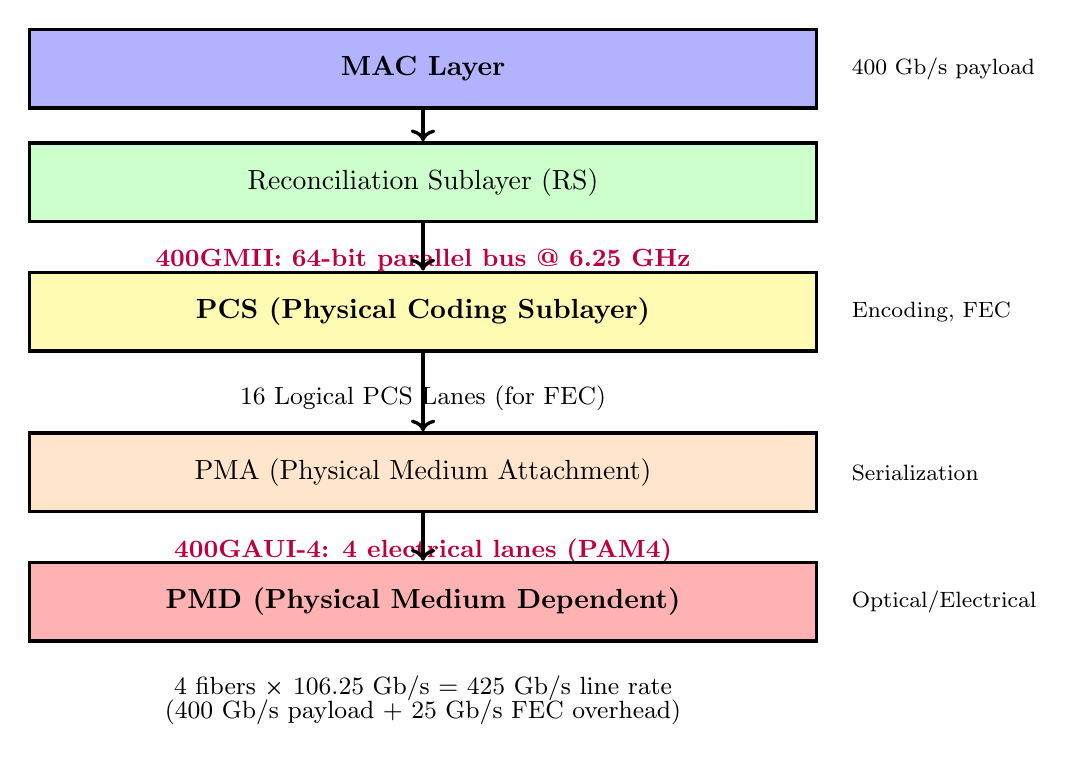
\begin{tikzpicture}[
    layer/.style={rectangle, draw=black, very thick, minimum width=10cm, minimum height=1cm, anchor=north},
    arrow/.style={->, very thick},
    label/.style={font=\footnotesize}
]

% MAC Layer
\node[layer, fill=blue!30] (mac) at (0,0) {\textbf{MAC Layer}};
\node[right=0.3cm of mac.east, anchor=west, label] {400 Gb/s payload};

% RS
\node[layer, fill=green!20, below=0.4cm of mac.south] (rs) {Reconciliation Sublayer (RS)};
\draw[arrow] (mac.south) -- (rs.north);

% 400GMII
\node[below=0.2cm of rs.south, font=\small\bfseries, color=purple] (gmii) {400GMII: 64-bit parallel bus @ 6.25 GHz};

% PCS
\node[layer, fill=yellow!30, below=0.6cm of rs.south] (pcs) {\textbf{PCS (Physical Coding Sublayer)}};
\node[right=0.3cm of pcs.east, anchor=west, label] {Encoding, FEC};
\draw[arrow] (rs.south) -- ++(0,-0.3cm) -- (pcs.north);

% 16 logical lanes
\node[below=0.3cm of pcs.south, font=\small] {16 Logical PCS Lanes (for FEC)};

% PMA
\node[layer, fill=orange!20, below=1cm of pcs.south] (pma) {PMA (Physical Medium Attachment)};
\node[right=0.3cm of pma.east, anchor=west, label] {Serialization};
\draw[arrow] (pcs.south) -- ++(0,-0.5cm) -- (pma.north);

% 400GAUI-4
\node[below=0.2cm of pma.south, font=\small\bfseries, color=purple] (gaui) {400GAUI-4: 4 electrical lanes (PAM4)};

% PMD
\node[layer, fill=red!30, below=0.6cm of pma.south] (pmd) {\textbf{PMD (Physical Medium Dependent)}};
\node[right=0.3cm of pmd.east, anchor=west, label] {Optical/Electrical};
\draw[arrow] (pma.south) -- ++(0,-0.3cm) -- (pmd.north);

% Output
\node[below=0.3cm of pmd.south, font=\small] {4 fibers × 106.25 Gb/s = 425 Gb/s line rate};
\node[below=0.6cm of pmd.south, font=\small] {(400 Gb/s payload + 25 Gb/s FEC overhead)};

\end{tikzpicture}
\caption{Complete 400G Ethernet architecture from MAC to fiber.}
\end{figure}
\end{fullwidth}

\section{Key Concepts Summary}

\subsection{Critical Numbers for 400G}

\begin{fullwidth}
\begin{table}
\centering
\begin{tabular}{lll}
\toprule
\textbf{Parameter} & \textbf{Value} & \textbf{Notes} \\
\midrule
\multicolumn{3}{l}{\textit{Data Rates}} \\
MAC Payload Rate & 400 Gb/s & Actual data throughput \\
Physical Line Rate & 425 Gb/s & Includes FEC overhead \\
Per-Lane Line Rate & 106.25 Gb/s & 425 Gb/s ÷ 4 lanes \\
\midrule
\multicolumn{3}{l}{\textit{Physical Layer}} \\
Number of Lanes & 4 & Independent optical/electrical lanes \\
Modulation & PAM4 & 4-level signaling \\
Symbol Rate & 53.125 GBaud & Symbols per second per lane \\
Bits per Symbol & 2 & PAM4 encoding \\
\midrule
\multicolumn{3}{l}{\textit{PCS Architecture}} \\
Logical PCS Lanes & 16 & For FEC processing \\
Physical Lanes & 4 & After bit-multiplexing \\
\midrule
\multicolumn{3}{l}{\textit{FEC Parameters}} \\
FEC Code & RS(544,514) & Reed-Solomon code \\
Total Symbols & 544 & Per codeword \\
Data Symbols & 514 & Payload \\
Parity Symbols & 30 & Redundancy \\
Correction Capability & 15 symbols & Per codeword \\
FEC Overhead & 5.8\% & (544-514)/514 \\
\bottomrule
\end{tabular}
\caption{Critical parameters for 400G Ethernet.}
\end{table}
\end{fullwidth}

\subsection{The Data Transformation Journey}

\begin{enumerate}
\item \textbf{64 parallel bits} (400GMII inside chip)
\item $\rightarrow$ \textbf{66-bit blocks} (64B/66B encoding)
\item $\rightarrow$ \textbf{257-bit blocks} (transcoding)
\item $\rightarrow$ \textbf{10-bit RS-FEC symbols} (strip sync, divide)
\item $\rightarrow$ \textbf{544-symbol codewords} (FEC encoding)
\item $\rightarrow$ \textbf{16 logical lanes} (FEC distribution)
\item $\rightarrow$ \textbf{4 physical lanes} (bit-multiplexing)
\item $\rightarrow$ \textbf{PAM4 symbols} (physical signaling)
\end{enumerate}

\section{Chapter Summary}

We've built a complete understanding of 400G Ethernet:

\begin{itemize}
\item \textbf{MAC Layer}: Creates frames, operates at 400 Gb/s payload
\item \textbf{400GMII}: 64-bit parallel bus inside chip
\item \textbf{PCS}: Encoding (64B/66B, 256B/257B), scrambling, FEC
\item \textbf{FEC}: RS(544,514) code, operates on 16 logical lanes
\item \textbf{PMA}: Bit-multiplexing (16 logical → 4 physical lanes)
\item \textbf{PMD}: PAM4 signaling, 4 physical lanes at 106.25 Gb/s each
\end{itemize}

With 400G mastered, the natural next step is 800G---which is essentially two of these 400G systems running in parallel.

% ============================================================================
% CHAPTER 2: 800G ETHERNET ARCHITECTURE  (skeleton --- to be expanded)
% ============================================================================

\chapter{800G Ethernet: Two 400G Systems in Parallel}

\marginnote{\textbf{Status:} Draft skeleton. Sections below are placeholders to
be filled in as the material is developed.}

\section{Introduction}

800G Ethernet builds directly on the 400G foundation from the previous chapter:
at its core, 800G is two 400G systems running in parallel. This chapter will
map that idea onto the IEEE 802.3 standards and the hardware that implements
them.

% TODO: Explain how 800G builds on 400G (800G = 2 x 400G DSPs in parallel)
% TODO: Reference the IEEE 802.3 Clause 172 specification

\section{The Dual-DSP Architecture}

% TODO: Explain the two-DSP design (e.g., 2 x 400G module DSPs)
% TODO: Include a diagram of the complete 800G system
% TODO: Cover 16 total FEC blocks (8 per DSP) and 8 optical lanes

\section{The 800GBASE-DR8 Standard}

% TODO: Cover the 800GBASE-DR8 physical layer standard
% TODO: 8 lanes x 106.25 Gb/s = 850 Gb/s line rate; 800 Gb/s payload after FEC
% TODO: OSFP vs QSFP-DD form factors

\section{Two-Flow PCS Architecture}

% TODO: Detail the 2x Clause 119 PCS architecture
% TODO: Block distribution between Flow 0 and Flow 1
% TODO: Each flow is an independent 400G PCS with its own FEC encoder

\section{Lane Distribution and Interleaving}

% TODO: Explain how data distributes across 8 physical lanes
% TODO: Logical lanes (16 per flow, 32 total) vs physical lanes (8 total)
% TODO: Lane alignment markers and synchronization

\section{Optical Module Architecture}

% TODO: Cover the OSFP module internals
% TODO: Pin constraints and signal routing
% TODO: Power budget and thermal considerations

\section{800G vs 400G Comparison}

% TODO: Comparison table (FEC blocks, lanes, line rate, payload rate, form factor)
% TODO: Highlight what changes and what stays the same

\section{Key Concepts Summary}

% TODO: Summarize critical 800G numbers and architecture decisions
% TODO: Add a "Critical Numbers for 800G" table similar to the 400G one

% ============================================================================
% CHAPTER 3: 1.6T ETHERNET ARCHITECTURE  (skeleton --- to be expanded)
% ============================================================================

\chapter{1.6T Ethernet: Scaling Beyond 800G}

\marginnote{\textbf{Status:} Draft skeleton. Sections below are placeholders to
be filled in as the material is developed.}

\section{Introduction}

1.6T (1.6 Tb/s) Ethernet is the next rung on the speed ladder above 800G. This
chapter will cover how the industry reaches 1.6T---primarily by moving to
higher per-lane rates (e.g., 212.5 Gb/s serial lanes) and/or wider lane counts,
along with the standards work in IEEE 802.3dj.

% TODO: Position 1.6T relative to 400G/800G; 1.6T = 2 x 800G or 8 x 200G lanes
% TODO: Reference the IEEE 802.3dj project

\section{Per-Lane Rate: 200G Lanes}

% TODO: Cover the move to ~212.5 Gb/s electrical/optical lanes
% TODO: PAM4 at higher baud vs alternative modulation (e.g., PAM6/coherent)
% TODO: Signal integrity and DSP implications of doubling per-lane rate

\section{FEC Evolution for 1.6T}

% TODO: Whether RS(544,514) still suffices or stronger/concatenated FEC is used
% TODO: Latency vs coding-gain trade-offs at 1.6T

\section{The 1.6TBASE Standards Family}

% TODO: Cover emerging 1.6TBASE-DR8 / -VR8 style variants (8 lanes x 200G)
% TODO: Form factors (OSFP-XD and successors)

\section{Lane Distribution and Interleaving}

% TODO: Logical vs physical lane mapping at 1.6T
% TODO: Alignment markers and skew management at higher rates

\section{Optical Module and Thermal Considerations}

% TODO: Power budget, thermal density, and co-packaged optics (CPO) direction

\section{1.6T vs 800G Comparison}

% TODO: Comparison table (per-lane rate, lane count, FEC, line rate, form factor)

\section{Key Concepts Summary}

% TODO: Summarize critical 1.6T numbers once the standard stabilizes

\end{document}
